%%%%%%%%%%%%%%%%%%%%%%%%%%%%%%%%%%%%%%%%%
% Beamer Presentation
% LaTeX Template
% Version 1.0 (10/11/12)
%
% This template has been downloaded from:
% http://www.LaTeXTemplates.com
%
% License:
% CC BY-NC-SA 3.0 (http://creativecommons.org/licenses/by-nc-sa/3.0/)
%
%%%%%%%%%%%%%%%%%%%%%%%%%%%%%%%%%%%%%%%%%

%----------------------------------------------------------------------------------------
%	PACKAGES AND THEMES
%----------------------------------------------------------------------------------------

\documentclass{beamer}

\mode<presentation> {

% The Beamer class comes with a number of default slide themes
% which change the colors and layouts of slides. Below this is a list
% of all the themes, uncomment each in turn to see what they look like.

%\usetheme{default}
%\usetheme{AnnArbor}
%\usetheme{Antibes}
%\usetheme{Bergen}
%\usetheme{Berkeley}
%\usetheme{Berlin}
%\usetheme{Boadilla}
%\usetheme{CambridgeUS}
%\usetheme{Copenhagen}
%\usetheme{Darmstadt}
%\usetheme{Dresden}
%\usetheme{Frankfurt}
%\usetheme{Goettingen}
%\usetheme{Hannover}
%\usetheme{Ilmenau}
%\usetheme{JuanLesPins}
%\usetheme{Luebeck}
\usetheme{Madrid}
%\usetheme{Malmoe}
%\usetheme{Marburg}
%\usetheme{Montpellier}
%\usetheme{PaloAlto}
%\usetheme{Pittsburgh}
%\usetheme{Rochester}
%\usetheme{Singapore}
%\usetheme{Szeged}
%\usetheme{Warsaw}

% As well as themes, the Beamer class has a number of color themes
% for any slide theme. Uncomment each of these in turn to see how it
% changes the colors of your current slide theme.

%\usecolortheme{albatross}
%\usecolortheme{beaver}
%\usecolortheme{beetle}
%\usecolortheme{crane}
%\usecolortheme{dolphin}
%\usecolortheme{dove}
%\usecolortheme{fly}
%\usecolortheme{lily}
%\usecolortheme{orchid}
%\usecolortheme{rose}
%\usecolortheme{seagull}
%\usecolortheme{seahorse}
%\usecolortheme{whale}
%\usecolortheme{wolverine}

%\setbeamertemplate{footline} % To remove the footer line in all slides uncomment this line
%\setbeamertemplate{footline}[page number] % To replace the footer line in all slides with a simple slide count uncomment this line

%\setbeamertemplate{navigation symbols}{} % To remove the navigation symbols from the bottom of all slides uncomment this line
}

\usepackage[T1]{fontenc}
\usepackage{graphicx} % Allows including images
\usepackage{booktabs} % Allows the use of \toprule, \midrule and \bottomrule in tables
\usepackage{hyperref} % Hyperlinks

\setbeamerfont{caption}{size=\footnotesize}

%----------------------------------------------------------------------------------------
%	TITLE PAGE
%----------------------------------------------------------------------------------------

\title[Introduction to Web Development]{SESA Web Development Shadow Class} % The short title appears at the bottom of every slide, the full title is only on the title page

\author{Saren Currie} % Your name
\institute[SESA] % Your institution as it will appear on the bottom of every slide, may be shorthand to save space
{
Software Engineering Students' Association \\ % Your institution for the title page
\medskip
\textit{saren@sarencurrie.com} % Your email address
}
\date{\today} % Date, can be changed to a custom date

\begin{document}

\begin{frame}
\titlepage % Print the title page as the first slide
\end{frame}

\begin{frame}
\frametitle{Overview} % Table of contents slide, comment this block out to remove it
\tableofcontents % Throughout your presentation, if you choose to use \section{} and \subsection{} commands, these will automatically be printed on this slide as an overview of your presentation
\end{frame}

%----------------------------------------------------------------------------------------
%	PRESENTATION SLIDES
%----------------------------------------------------------------------------------------

%------------------------------------------------
\section{Introduction} % Sections can be created in order to organize your presentation into discrete blocks, all sections and subsections are automatically printed in the table of contents as an overview of the talk

%------------------------------------------------

\subsection{What you need} % A subsection can be created just before a set of slides with a common theme to further break down your presentation into chunks

\begin{frame}
\frametitle{Pick a browser}

\begin{figure}
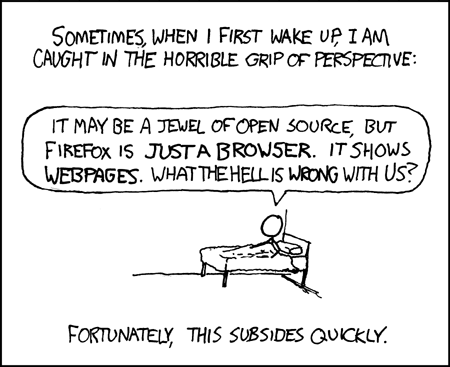
\includegraphics[width=0.8\linewidth]{img/perspective.png}
\end{figure}

\end{frame}

%------------------------------------------------

\begin{frame}
\frametitle{Essential Tools for Web Development}
\begin{itemize}
\item A web browser (Chrome, Firefox, Safari)
\item A text editor (Sublime, TextMate, WebStorm or try VS Code)
\item Version control
\item Useful Sites
\begin{itemize}
	\item \href{http://google.com}{Google}
	\item \href{http://www.stackoverflow.com/}{Stackoverflow}
	\item \href{http://www.w3schools.com}{w3schools (basic guides and documentation)}
	\item \href{https://developer.mozilla.org/en-US/docs/Web}{Mozilla Developer Network (more advanced documentation)}
\end{itemize}
\item Time
\end{itemize}
\end{frame}

%------------------------------------------------

\section{The Basics}
\subsection{HTML}

\begin{frame}
\frametitle{HTML Elements}
\begin{block}{Tags}
Defines what each element is. For example, headings: \textbf{<h1>}; \textbf{<h2>} etc., paragraphs: \textbf{<p>}, containers: \textbf{<div>}; \textbf{<span>}.
\begin{figure}

\includegraphics[width=0.8\linewidth]{img/tags.png}
\end{figure}
\end{block}

\begin{block}{Attributes}
Allow you to assign useful information to each element. Eg: class, id
\end{block}

\begin{block}{Contents}
What goes inside the tags to make a complete element. These can be nested.
\end{block}

All of these go together to make an element.

\texttt{<a class="home-link nav" id="home\_link" href="/">Home</a>}

\end{frame}

%------------------------------------------------
\subsection{CSS}
%------------------------------------------------

\begin{frame}
\frametitle{CSS}

\begin{block}{Selectors}
Use tags and properties to define which element(s) the css statement applies to using class, id or others. Classes are prepended with . ids with \# and tags with nothing.

The selectors: \texttt{a}, \texttt{.nav}, \texttt{\#home\_link} and \texttt{a.nav.home-link\#home\_link} would all apply to the example from the previous page.

A list of many possible selectors is available \href{http://en.wikipedia.org/wiki/Cascading_Style_Sheets\#cite_ref-6}{here}.
\end{block}

\begin{block}{Declarations}
After the selector (in a set of braces \{\}), a list of declarations define visual information about the element(s) the selectors refer to in the format \texttt{property: value;}
\end{block}

Here's some example css

\texttt{a.nav \{ background: \#38a712; padding: 20px 40px; \}}

\end{frame}

%------------------------------------------------

\begin{frame}
\frametitle{The Box Model}

\begin{figure}
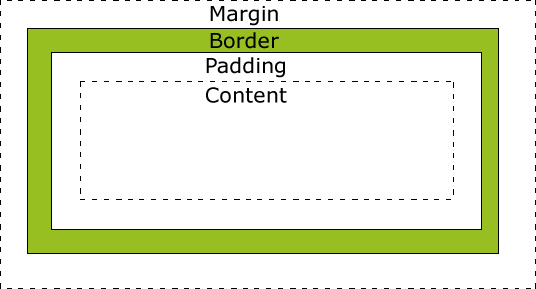
\includegraphics[width=0.5\linewidth]{img/box-model.png}
\end{figure}

\begin{itemize}
\item The box model is essentially how css handles the geometry of each element.
\item The content and padding are coloured if/when you set the background colour, the border is coloured if/when you define a border size style and colour, and the margins are not coloured.
\item The size of each part of the box model can be defined in your css.
\begin{itemize}
\item \textbf{All sides:} \texttt{margin: 5px;}
\item \textbf{Vertical/horizontal:} \texttt{padding: 5px 10px;}
\item \textbf{Top/Right/Bottom/Left:} \texttt{border-width: 1px 2px 3px 4px;}
\end{itemize}
\end{itemize}
\end{frame}

%------------------------------------------------
\section{Let's Make Something!}
%------------------------------------------------

\begin{frame}
\frametitle{Play Along at Home}

\begin{block}{Using git}
The source code for the demonstration project (as well as these slides) is available on github.

\texttt{git clone https://github.com/ausesa/html-css-shadowclass.git}
\end{block}

\begin{block}{Direct download}
Alternatively, go to \href{https://github.com/ausesa/html-css-shadowclass/releases}{https://github.com/ausesa/html-css-shadowclass/releases} for a direct download of the source code for the demonstration project.
\end{block}

\end{frame}

%----------------------------------------------------------------------------------------

\end{document} 
